\chapter{Experiment 2: validation of remote detection of emotions}
\label{ch:experiment2}

The experiment described in this chapter, the second one conducted, aimed at validating the proposed approach for remote detection of emotions, described in the objectives of this thesis (see Section \ref{sec:contributions}, on page \pageref{sec:contributions}). The approach uses remotely acquired signals, namely heart rate (HR) and facial actions (FA), to create a user-tailored model, i.e. trained neural network, able to detect emotional states of boredom and stress of a given subject. The approach is composed of two phases: training (or calibration) and testing. In the training phase, the model is trained using a user-tailored approach, i.e. data from subject $S_a$ playing 3 calibration games (Mushroom, Platformer and Tetris) is used to create model $M_a$. The result of the training phase is a user-tailored model, i.e. model $M_a$, which is a trained neural network aimed to be used on subject $S_a$. The testing phase happens in a game session involving subject $S_a$ playing any ordinary, non-calibration game, e.g. Super Mario. During the testing phase, subject's $S_a$ signals are remotely acquired and fed into the previously trained model $M_a$, which outputs the estimated emotional state of subject $S_a$ for that particular testing game.

In summary, this experiment was intended to answer the following research question:

\begin{fquote}
How accurate is an emotion detection approach that uses remotely acquired signals, i.e. heart rate and facial actions, as input of a machine learning model, i.e. neural network, that was trained on a user-tailored basis (one subject produces one model) using calibration games as emotion elicitation?
\end{fquote}

The overall hypothesis of this experiment is that the accuracy of the model during the testing phase is acceptable. It validates and proves the proposed approach as feasible. The next sections present the experiment, detailing the participants, structure and results, followed by a discussion and a conclusion.

%%%%%%%%%%%%%%%%%%%%%%%%%%%%%%%%%%%%%%%%%%%%%%%%%%%%%%%%%%%%%%%%%%%%%%%%%%%%%%%%%%%%%%%
\section{Participants}
%%%%%%%%%%%%%%%%%%%%%%%%%%%%%%%%%%%%%%%%%%%%%%%%%%%%%%%%%%%%%%%%%%%%%%%%%%%%%%%%%%%%%%%

Sixty two ($N=62$) adult participants of both genders (38.7\% female, 61.3\% male) with different ages (19 to 66, mean 27.2, SD 7.2) and different gaming experience gave their informed and written consent to participate in the experiment. The study population consisted of staff members and students of the University of Sk\"ovde, as well as citizens of the community/city.

When asked how skilled subjects believe they are at playing video games, 6 subjects (9.7\%) reported no skill, 19 (30.6\%) reported not very skilled, 25 (40.3\%) reported moderately skilled and 12 (19.9\%) reported very skilled. When asked the number of hours per week they had played any type of video game over the last year, 25 subjects (40.3\%) reported more than 10, 7 (11.3\%) reported 5 to 10, 6 (9.7\%) reported 3 to 4, 5 (8.1\%) reported 1 to 3, 10 (16.1\%) reported 0 to 1, and 9 (14.5\%) reported no activity.

Those numbers indicate that the sample population has a diversity of ages, gaming experience and playing frequency. Such diversity provides heterogeneous data that allows a more realistic and broad analysis of the proposed method.

%%%%%%%%%%%%%%%%%%%%%%%%%%%%%%%%%%%%%%%%%%%%%%%%%%%%%%%%%%%%%%%%%%%%%%%%%%%%%%%%%%%%%%%
\section{Method}
\label{sec:experiment2-method}
%%%%%%%%%%%%%%%%%%%%%%%%%%%%%%%%%%%%%%%%%%%%%%%%%%%%%%%%%%%%%%%%%%%%%%%%%%%%%%%%%%%%%%%

The following sections present the experiment structure and the methods employed to collect and analyze data.

%%%%%%%%%%%%%%%%%%%%%%%%%%%%%%%%%%%%%%%%%%%%%%%%%%%%%%%%%%%%%%%%%%%%%%%%%%%%%%%%%%%%%%%
\subsection{Experimental design and setup}

Subjects were seated in front a computer, alone in the room, while being recorded by a camera and measured by a heart rate sensor, as illustrated in Figure \ref{fig:experiment2-setup}. The camera was attached to a tripod placed in front of the subjects at approximately 0.6m of distance; the camera was slightly tilted up. A spotlight, tilted 45$^{\circ}$ up, placed at a distance of 1.6m from the subject and 45cm higher than the camera level, was used for illumination; no other light source was active during the experiment.

\begin{figure}[ht]
\centering
  \begin{subfigure}[b]{0.5\textwidth}
    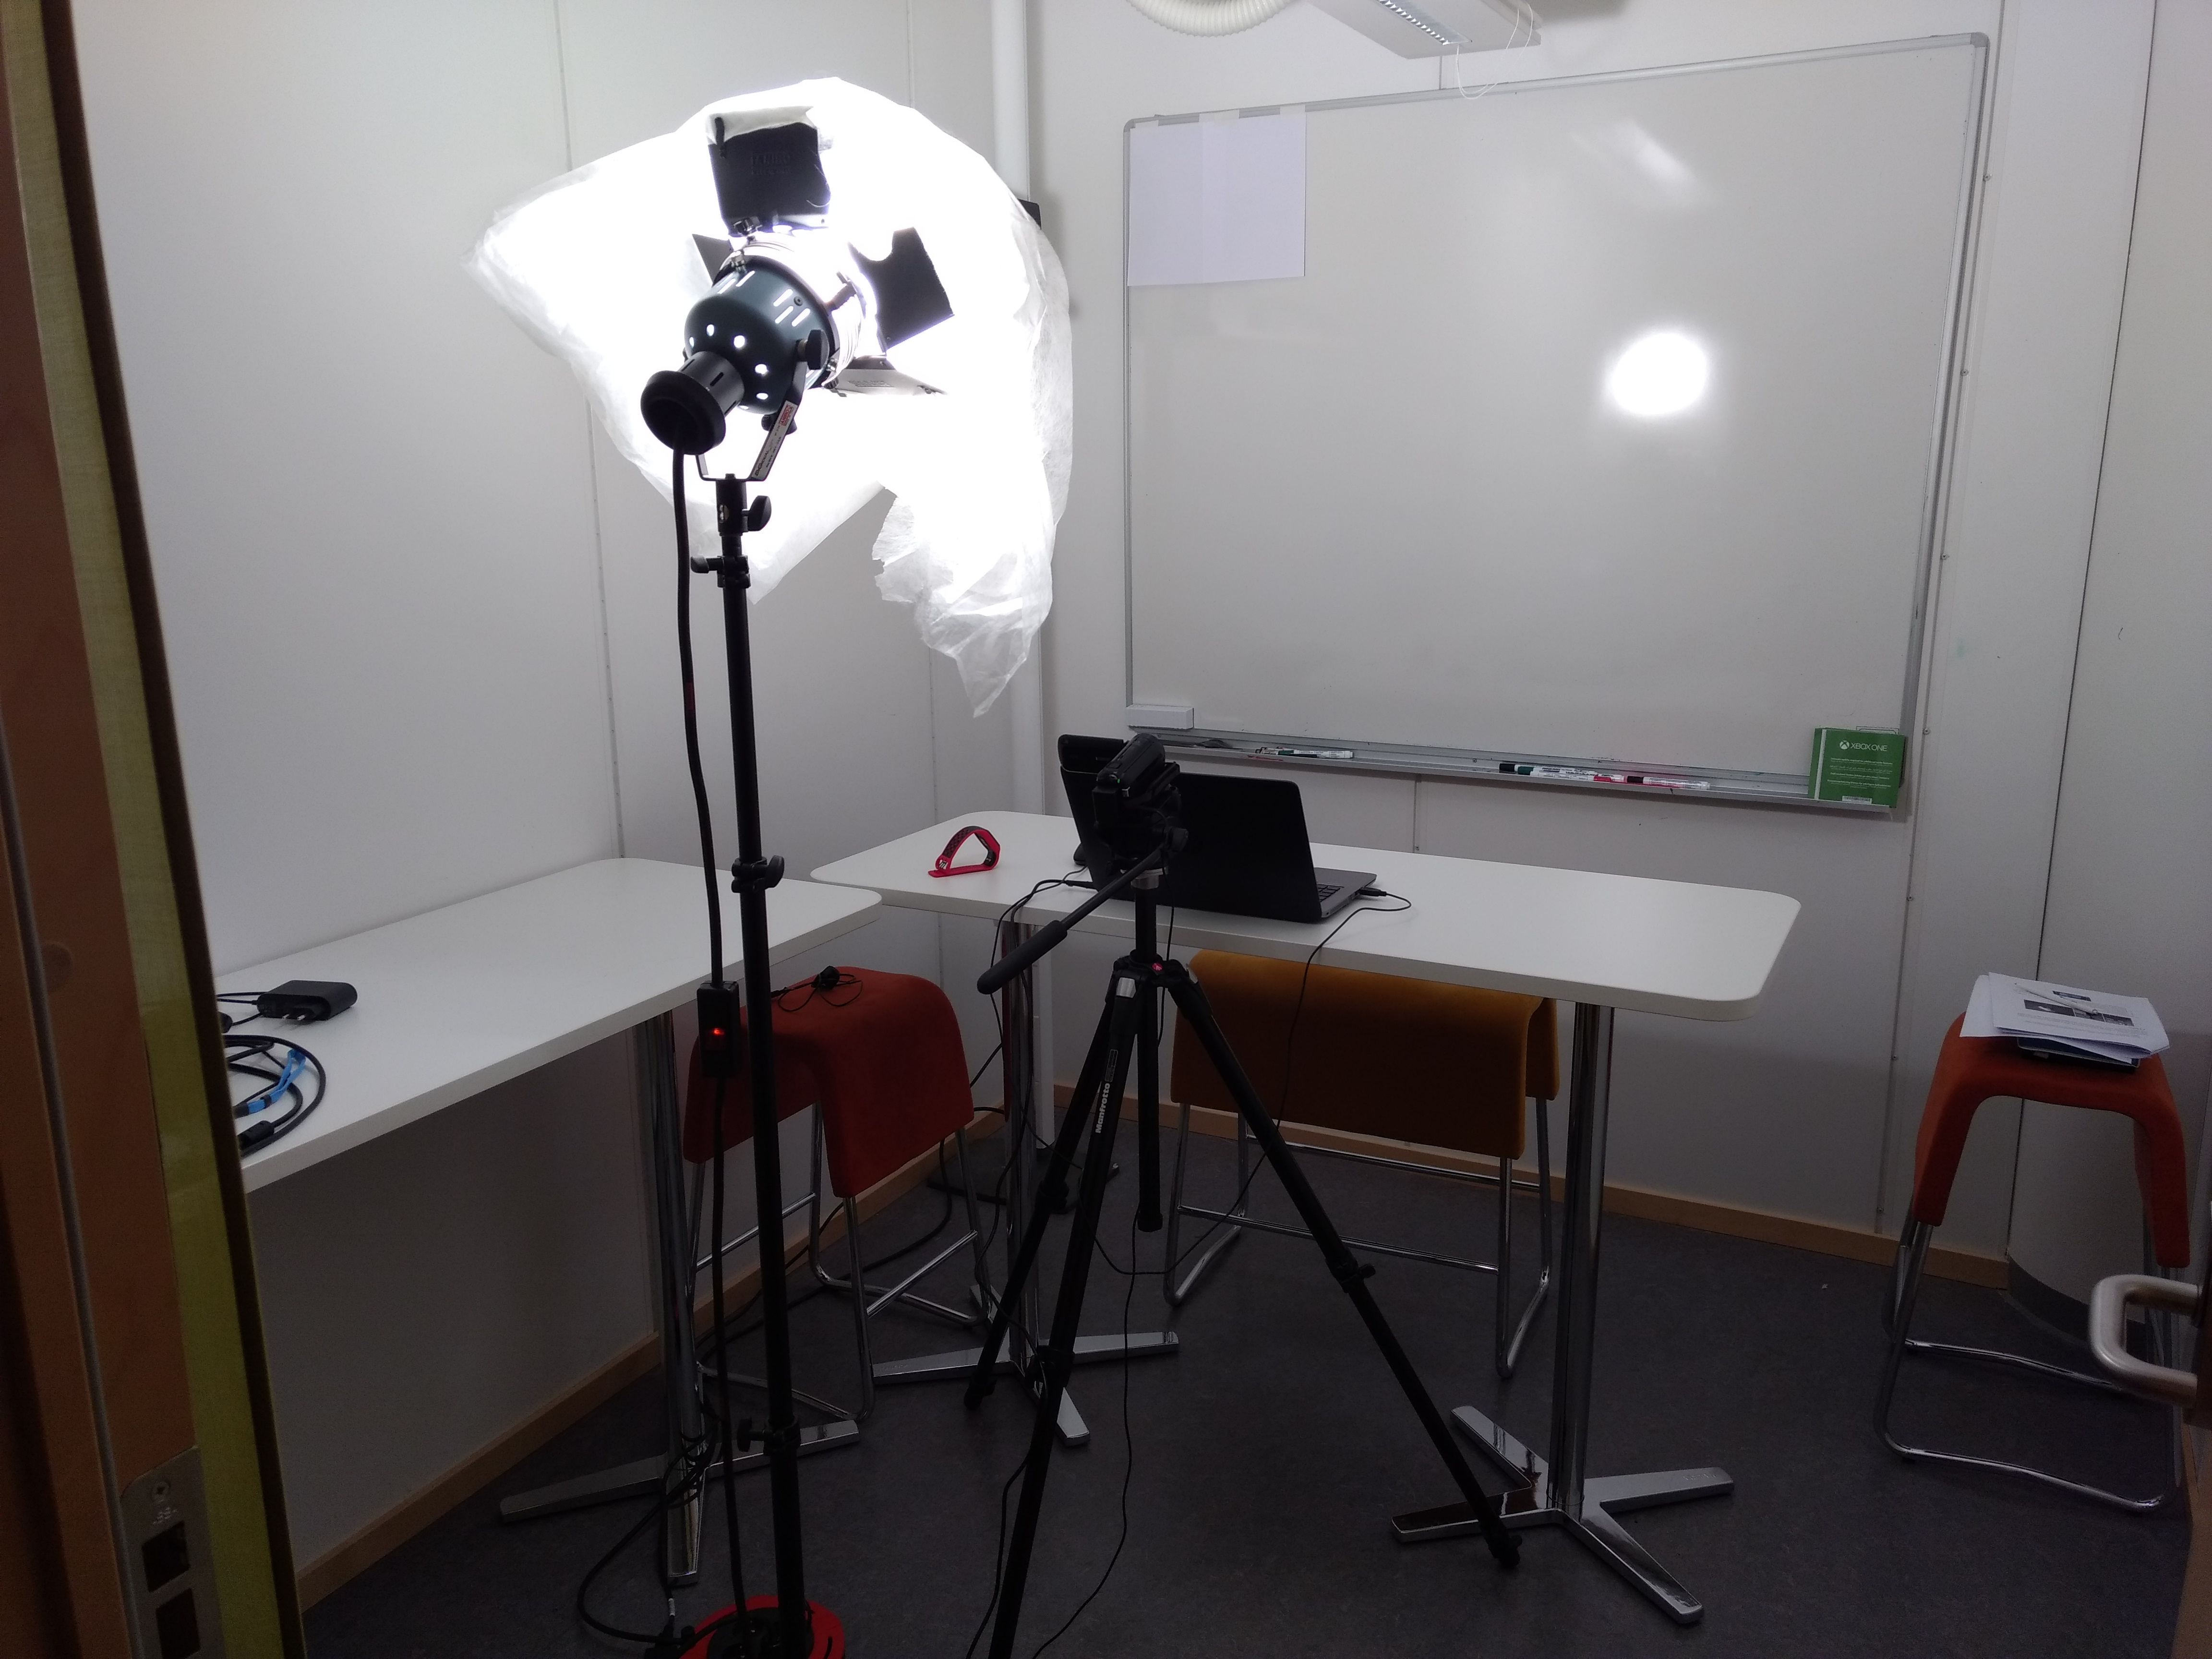
\includegraphics[width=0.95\textwidth]{figures/experiment2-setup-overall}
    \caption{}
    \label{fig:experiment2-setup-overall}
  \end{subfigure}%
  \begin{subfigure}[b]{0.5\textwidth}
    \centering
    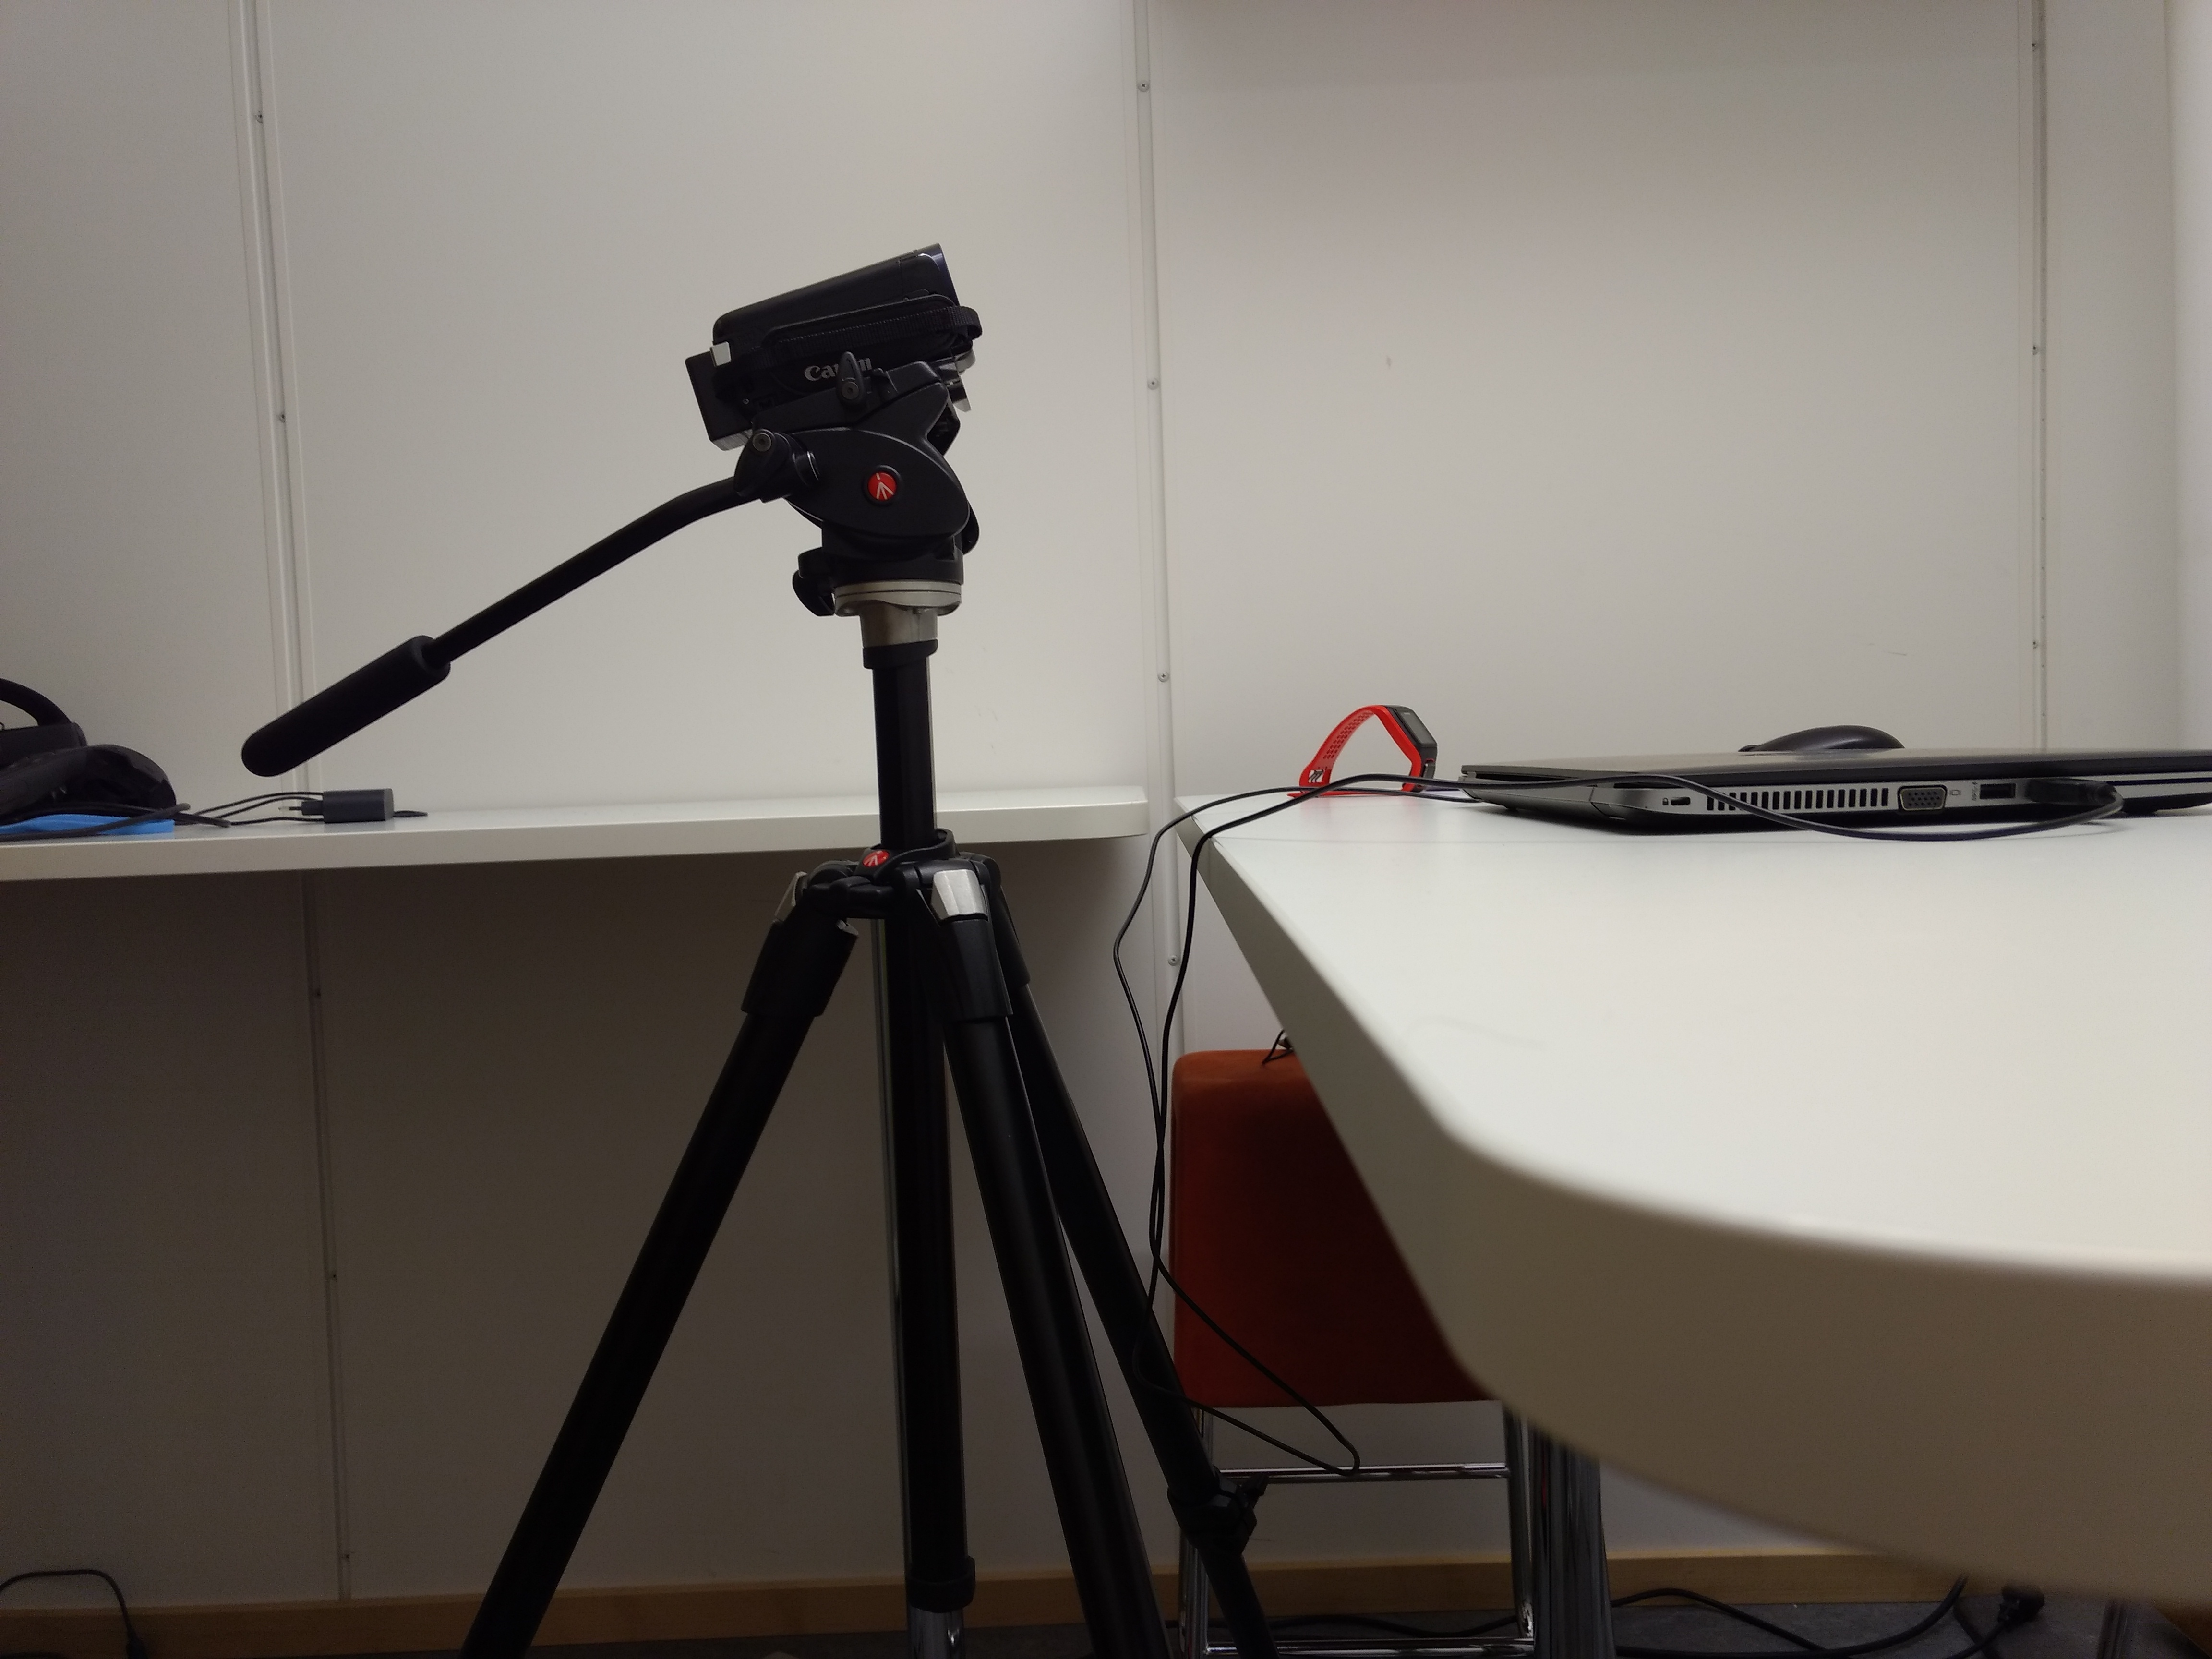
\includegraphics[width=0.95\textwidth]{figures/experiment2-setup-camera}
    \caption{}
    \label{fig:experiment2-setup-camera}
  \end{subfigure}
  \caption{Experiment setup. (a) Position of equipment, showing computer, camera, and external light source. (b) Highlight of the video camera and it angulation.}
  \label{fig:experiment2-setup}
\end{figure}

Participants were each recorded for about 45 minutes on average during two (uninterrupted) parts of the experiment, i.e. calibration and testing phase, as illustrated by Figure \ref{fig:experiment2-parts}. The calibration phase, aimed at gathering data for training a user-tailored model, subjects played 3 games (described in Section \ref{sec:experiment2-calibration-games}). Each of those games was followed by a questionnaire related to the game and stress/boredom levels. Games were also followed by a 138 seconds rest period where subjects listened to calm classic music. The testing phase, aimed at gathering data to test the accuracy of the user-tailored model, subjects played 7 levels of an evaluation game, i.e. Infinite Mario (described in Section \ref{sec:experiment2-evaluation-game}).

In the calibration phase, games were carefully designed to start with a difficulty level that is significantly low, which is expected to lead the player to an immediate state of boredom. As time progresses, the difficulty level increases linearly. As the difficulty level continues to rise, at certain point the game will become too hard to be managed by the subject, which eventually results in a ``game over" state. Moments before that point the subject should reach his/her stress peak during gameplay. It is expected that each player experiences three distinct states during the gameplay of each game: boredom (low challenge/stress) at the beginning, flow (ideal challenge/stress) after the beginning and before the final moments, and stress (high challenge/stress) at the end. The order in which the games were played was randomized among subjects during the calibration phase of the experiment.

\begin{figure}[ht]
  \centering
  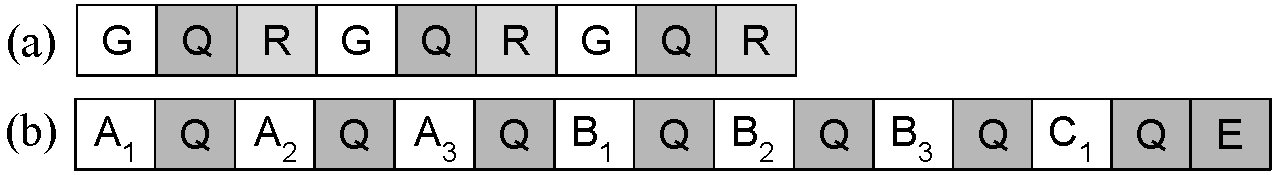
\includegraphics[width=\textwidth]{figures/experiment2-parts}
  \caption{Experiment setup}
  \label{fig:experiment2-parts}
\end{figure}

In the testing phase, subjects played 3 batches of Infinite Mario levels: batches $A$, $B$ and $C$ containing 3, 3 and 1 level each, respectively. Except for level $C_1$ in batch $C$, levels in batches $A$ and $B$ were designed to present an increase in difficulty within the batch, so levels $A_1$ and $B_1$ are expected to be less difficult/challenging than levels $A_3$ and $B_3$, for instance. Similarly levels in batch $B$ were designed to be more challenging than levels in batch $A$, also following an increase in difficulty. Consequently levels $B_i$ are expected to be slightly more difficult/challenging than levels $A_i$. This pattern is intended to mimic the balance curve of a commercial game, where levels, and game parts, commonly tend to increase its difficulty as the game story progresses. In order to ensure subjects would experience some level of boredom during the testing phase, which is required for the evaluation of the proposed method, levels $B_1$ and $C_1$ were designed using Mario's auto-scrolling camera mechanics. In such configuration, the player has no control of the speed of the level. This mechanic is expected to induce boredom, since the player experienced allegedly challenging (and fun) levels previously and is now unable to move using any desired speed. After each level, subjects answered a questionnaire about how boring/stressful the game level just played was. The order in which the levels were played was not randomized among subjects during the testing phase of the experiment. As a consequence, all subjects played the evaluation game in the same order: levels $A_1$ to $A_3$, followed by levels $B_1$ to $B_3$, finally followed by level $C_1$.

After subjects finished playing the last level in the testing phase, i.e. level $C_1$, they answered a final questionnaire about age and gaming experience/profile. Before starting the experiment, participants received instructions from a researcher that they should play a few games, answer questionnaires after each game and rest when instructed; they were told that their gaming performance was not being evaluated, that they should not give up in the middle of the games, that a time limit exists for some levels to prevent them from playing for too long, and that they should remain seated during the whole process.

\subsection{Calibration games}
\label{sec:experiment2-calibration-games}

The three games used as calibration games, i.e. Mushroom, Platformer and Tetris, were already described in details in Section \ref{sec:experiment1-games-elicitation} (on page \pageref{sec:experiment1-games-elicitation}). The present experiment used exactly the same calibration games used in the first conducted experiment (see Chapter \ref{ch:experiment1}). The games are 2D and casual-themed, played with mouse or keyboard in a web browser. They were carefully designed to provoke boredom at the beginning and stress at the end, with a linear progression between the two states.

\subsection{Evaluation game}
\label{sec:experiment2-evaluation-game}

%Pedersen, C.; Togelius, J. & Yannakakis, G. N. Modeling player experience in Super Mario Bros. 2009 IEEE Symposium on Computational Intelligence and Games, IEEE, 2009, 132-139

%Pedersen, Christopher, Julian Togelius, and Georgios N. Yannakakis. "Modeling player experience for content creation." IEEE Transactions on Computational Intelligence and AI in Games 2.1 (2010): 54-67.

%Shaker, N.; Asteriadis, S.; Yannakakis, G. N. & Karpouzis, K. A game-based corpus for analysing the interplay between game context and player experience. Affective Computing and Intelligent Interaction, Springer, 2011, 547-556

% Shaker, N.; Yannakakis, G. N. & Togelius, J. Feature analysis for modeling game content quality. 2011 IEEE Conference on Computational Intelligence and Games (CIG'11), IEEE, 2011, 126-133

The game used in the evaluation phase of the experiment is a modified version\footnote{The version of the game used in the experiment is a HTML5, web-based version built by Robert Kleffner, available at: https://github.com/robertkleffner/mariohtml5. Robert ported to HTML5 the original Java version created by Markus Persson. Source code of both versions, Robert's and Markus', are in the public domain. The source code of the final version used in this experiment is available at: https://fernandobevilacqua.com/link/phd-experiment2} of Markus Persson's Infinite Mario, a public domain clone of Nintendo's platform game \textit{Super Mario Bros}. In the case of this experiment, the game is played with a keyboard in a web browser. Infinite Mario has been widely mentioned in the literature, including studies involving modeling of player experience \parencite{pedersen2009modeling,pedersen2010modeling,shaker2011game} and detection of affective states \parencite{shaker2011feature}.

\begin{figure}[h]
  \centering
  
\includegraphics[width=.32\textwidth]{figures/mario-overground}\hfill
  
\includegraphics[width=.32\textwidth]{figures/mario-underground}\hfill
  
\includegraphics[width=.32\textwidth]{figures/mario-castle}
  \caption{Screenshots from Infinite Mario. From left to right, level types \textit{Overground}, \textit{Underground} and \textit{Castle}, respectively.}
  \label{fig:experiment2-infinite-mario}
\end{figure}

The gameplay in Super Mario, consequentially in Infinite Mario as well, consists of controlling the main character, Mario, along the level. Mario can move left or right, jump, run, duck, and throw fireballs (if the power-up \textit{Flower} has been collected). The objective of the game is to complete each level, which is accomplished by traversing it from left to right until the ``end of level" checkpoint is reached. Mario can be in three different states: small, big, and power-up. If Mario is small, any interaction with enemies differently from landing on top of them after a jump results in Mario getting killed immediately. If Mario is big, the same ``wrong" interaction with enemies causes Mario to get hurt and transform into the small state. If Mario is in the power-up state, the ``wrong" interaction with enemies causes Mario to get hurt and transform into the big state. Consequently keeping Mario in the big or power-up state is a strategic advantage to prevent kills that likely calms the player, i.e. relaxed. On the other hand keeping Mario in the small state is less beneficial since mistakes are fatal, so it is likely that players feel anxious/stressed in such conditions.

Along the level, Mario might encounter enemies, which can be killed or ignored. Mario can kill enemies by jumping and landing on top of them, which is rewarded with score points. Some enemies, e.g. Koopa Troopa (a sort of turtle), leave a shell behind when killed by Mario. The shell can be picked up by Mario and carried around, serving as a weapon when released. Levels might also contain terrain obstacles of varying sizes, e.g. gaps, that must be jumped over. If Mario falls in a gap, he dies immediately. Mario can also find collectable items, i.e. coins and power-ups, or interactable items, e.g. blocks. Mario collects items by touching them, i.e. a collected coin results in score points. Collectable items might be visible in the level or hidden inside interactable items, e.g. blocks. Mario interacts with blocks by bumping into them from below, e.g. jumping and hitting Mario's head on the bottom of a block destroys it. A destroyed block might give a collectable item as a reward, e.g. coin, \textit{Mushroom} (Mario transitions to big state) or \textit{Flower} (Mario transitions to power-up state).

During gameplay, information about Mario, the score and the current level is displayed on the top of the screen. The information includes the number of lives Mario has left (to complete that level), the level score, the number of coins collected (collecting 100 coins results in an extra life), the name of the current level, and the amount of time available to complete the level (constantly ticking down). When the time remaining to complete the level reaches the 60 seconds mark, a hurry up SFX is played, then the background music starts to play in a faster tempo. Unless informed otherwise, all levels of Infinite Mario in the experiment start with 3 lives and 200 seconds of available time. Every time Mario dies, the time remaining to complete the level is reset to its initial value, e.g. 200 seconds.

Originally Infinite Mario procedurally generates all its gameplay content, e.g. level design and position of items/enemies. This behavior is not desired for the experiment, since all subjects should experience the same Mario levels. Additionally subjects should feel stressed and bored in game at some points, so the proposed emotion detection method can be properly evaluated when detecting such moments. As a consequence, Infinite Mario was adapted and tweaked to fit as an ideal evaluation game in the experiment. Procedural content generation was constrained by a seed and a set of parameters was introduced to control how content is created, e.g. length of the level, amount and width of terrain obstacles, e.g. gaps and platforms, availability of coins and power-ups, among others. It ensured that all subjects experienced the exactly same levels.

Previous works using Infinite Mario \parencite{pedersen2009modeling,pedersen2010modeling} have shown a correlation between anxiety and 1) difficulty of jumping, e.g. overcoming obstacles, and 2) gap width. There is also a correlation between boredom and the width of gaps, i.e. the wider the gap, the less boring the level is. Based on those findings and the guidance provided by game design experts, the Mario levels used in the experiment were adjusted according to the description presented in Table \ref{table:experiment2-mario-levels}. Column \textit{Level} refers to the level name/number. Column \textit{Type} refers to the overall visual representation of the level. Possible types are \textit{Overground} (open sky and green landscape), \textit{Underground} (closed ceiling, dirt-like environment), and \textit{Castle} (closed ceiling with bricks resembling the interior of a castle). Each level type features different background music and visual elements, as illustrated in Figure \ref{fig:experiment2-infinite-mario}. Column \textit{Emotion} refers to the expected emotional state most subjects will experience. Finally column \textit{Adjustments} refer to the constraints used to generate the levels content.

\begin{landscape}
\begin{table*}
    \centering
    \caption{Levels of Infinite Mario and adjustments performed to induce a particular emotional state from them.}
    \label{table:experiment2-mario-levels}
    \begin{tabular}[l]{@{}cllp{9.5cm}}
        \hline
            \textbf{Level} & \textbf{Type} & \textbf{Emotion} & \textbf{Adjustments} \\
        \hline
            $A_1$ & Overground  & Any & Reduced number of interactable/collectable items and terrain obstacles; no power-ups; only 2 enemies and 1 gap (with width of Mario himself); Mario starts in big state. \\
            $A_2$ & Underground & Any & Regular number of interactable/collectable items, terrain obstacles, power-ups and enemies. Mario starts in small state. \\
            $A_3$ & Castle      & Stress  & Several gaps (with varying widths); reduced number of interactable items; no collectables/power-ups; several enemies; reduced time to complete level. Mario remains in small state. Mario starts with 5 lives. Available level time is 80 seconds. \\
            $B_1$ & Overground  & Boredom & Auto-scrolling camera; reduced number of interactable/collectable items; few terrain obstacles; no gaps, power-ups, or enemies. Mario remains in big state. \\
            $B_2$ & Underground & Any & Regular number of interactable/collectable items, terrain obstacles, power-ups and enemies. Mario starts in small state. \\
            $B_3$ & Castle      & Stress  & Several gaps (with varying widths); reduced number of interactable items; no collectables/power-ups; several enemies; reduced time to complete level. Mario remains in small state. Mario starts with 5 lives. Available level time is 80 seconds. \\
            $C_1$ & Overground  & Boredom & Auto-scrolling camera; reduced number of interactable/collectable items; few terrain obstacles; no gaps, power-ups, or enemies. Mario remains in big state. \\
        \hline
    \end{tabular}
\end{table*}
\end{landscape}

Level $A_1$ is an introduction to the game to make subjects familiar with the mechanics, e.g. move, jump, collect items. Levels $A_2$ and $B_2$ were designed to be regular Mario levels with a compelling and enjoyable challenge scale.

Levels $A_3$ and $B_3$ were designed to be more stressful. Those levels present more enemies and several gaps, which are wider than usual. The absence of power-ups, the number of challenges, i.e. enemies and wide gaps, and the fact that Mario is continuously in small state should force subjects to better time actions, e.g. jump, and constantly pay attention to surroundings. Those levels also use the \textit{Castle} type, which is usually associated with ``boss levels" in Super Mario (commonly more challenging). Finally levels $A_3$ and $B_3$ have an available time of 80 seconds to be finished, a considerably lower value compared to 200 seconds in other levels. As a consequence, after 20 seconds of gameplay, the hurry up SFX is played and the background music starts to play faster. Such configuration is likely to cause an emotional state of stress.

Differently, levels $B_1$ and $C_1$ were designed to be more boring. Those levels present an auto-scrolling camera mechanic, where the camera automatically traverses the level independently of how Mario movements. The speed of the auto-scrolling camera has been adjusted to be constant, however in a slow pace. Additionally the reduced number of interactable/collectable items, the existence of few terrain obstacles, and the absence of gaps, power-ups and enemies is likely to cause an emotional state of boredom. Additionally levels $B_1$ and $C_1$ are very similar visually, which might make subjects perceive level $C_1$ as a repetition of level $B_1$. If that happens, subjects might perceive level $B_1$ as even more boring, since the level topology is already known and the player is unable to move the camera in a faster pace.

As previously mentioned, levels were adjusted and play-tested by game design experts. It ensured that the content of all levels and the constraints/modifications applied to them did not affect the subject's perception of playing a clone of a Mario. For instance the order in which the levels were played, i.e. repeating the pattern of an overground, then an underground and finally a castle level, was kept as an important element. It should mimic the expected world progression of the original Mario game, where the final level of a particular world is usually a castle level with a boss. Finally particular attention was invested to make Infinite Mario in-level difficulty as different as possible from the linear difficulty progression present in the three calibration games. The aim was to make Infinite Mario as similar to Super Mario as possible respecting the content constraints mentioned previously.

\subsection{Data collection}

During the whole experiment, subjects were recorded using a Canon Legria HF R606 video camera. All videos were recorded in color (24-bit RGB with three channels $\times$ 8bits/channel) at 50p frames per second (fps) with pixel resolution of 1920 $\times$ 1080 and saved in AVCHD-HD format, MPEG-4 AVC as the codec. At the same time, subject's HR was measured by a TomTom Runner Cardio watch (TomTom International BV, Amsterdam, Netherlands). The watch was placed on the left arm, approximately 7cm away from the wrist, like a regular wrist watch. The use of the watch was unobtrusive, so it did not affect the movements of the subjects, who could still use both hands to play the games. The watch recorded the HR at 1 Hz.

In the calibration phase of the experiment, subjects answered a questionnaire after each game in order to provide a self-reported level of stress and boredom. The questionnaire had six questions: the first four were a 5-point Likert scale related to how the player felt regarding stress/boredom at the beginning/end of each game (1: not stressed/bored at all, 5: extremely stressed/bored); a question to identify the part of the game that best describes the moment the subject enjoyed the most (very beginning, after beginning and before middle, middle, after middle and before end, very end); finally a question asking if the subject understood the game. In the testing phase of the experiment, subjects answered a questionnaire after each level of Infinite Mario to provide a self-reported level of stress and boredom about the played level. The questionnaire had two questions, one about stress and one about boredom, both with a 5-point Likert scale related to how stressed/bored the player felt while playing the level (1: not stressed/bored at all, 5: extremely stressed/bored). Finally before the end of the experiment, subjects answered a questionnaire with ten questions related to: age; gender; number of hours per week spent with games over the last year (question from the video game experience questionnaire \parencite{unsworth2015playing}); how proficient or skilled the subject believe being at playing video games (question from the Survey of Spatial Representation and Activities - SSRA \parencite{terlecki2005important}); familiarity with puzzle, platform, Tetris and Mario games; current state of mind compared to other days (e.g. normal, unusually stressed, etc.); and familiarity with the research related to the experiment (unfamiliar, not very familiar, moderately familiar, very familiar).

%%%%%%%%%%%%%%%%%%%%%%%%%%%%%%%%%%%%%%%%%%%%%%%%%%%%%%%%%%%%%%%%%%%%%%%%%%%%%%%%%%%%%%%
\subsection{Data preprocessing}

The video recordings of the experiment were pre-processed to allow the extraction of training and validation data. The process involved the extraction of the parts containing the interaction with games/levels and the discard of noisy frames. The pre-process procedure is notably similar to the one described in Section \ref{s:experiment1-study4-feature-analysis} (on page \pageref{s:experiment1-study4-feature-analysis}). The periods where subjects were playing the available games and levels were extracted from the video recordings. The pre-processing of the calibration phase resulted in 3 videos per subject, denoted $C_{s,i}$ where $s$ is the $s$-th subject and $i \in \{1, 2, 3\}$ represents a calibration game. The initial 45 seconds of any given video $C_{s,i}$ were removed since they were deemed noisy regarding emotional information. The remaining of the video was then divided into 3 pieces, from which the first and the last were selected as $H_0$ and $H_1$, respectively. The middle part was discarded because its emotional state is unknown. Segments $H_0$ and $H_1$ represent the boring and stressful parts of the calibration games, respectively. The pre-processing of the testing phase resulted in 7 segments per subject, denoted $M_{s,j}$ where $s$ is the $s$-th subject and $j \in \{1, 2, ..., 7\}$ represents a level of Infinite Mario. Video segment $M_{1,4}$, for instance, represents the recording of subject 1 playing level $B_1$.

Pre-processing of all recordings resulted in 13 video segments per subject: 3 segments $H_0$ (one per calibration game), 3 segments $H_1$ (one per calibration game), and 7 segments $M$ (one per level of Infinite Mario). Considering all subjects, the pre-processing of the calibration phase resulted in $N=186$ pairs of $H_0$ and $H_1$ video segments (3 calibration games $\times$ 62 subjects, resulting in 186 segments $H_0$ and 186 segments $H_1$). The testing phase resulted in $N=434$ video segments $M$ (7 levels of Infinite Mario $\times$ 62 subjects).

\subsection{Features extraction}

Features used in the classification model were extracted remotely via analysis of the video segments of each subject. Detailed information regarding how each feature is extracted, calculated, aggregated, and the reasoning why it is used has been previously presented in Sections \ref{s:study4} and \ref{s:experiment1-study5} (pages \pageref{s:study4}\ and \pageref{s:experiment1-study5}, respectively).

In total 8 features, denoted $F_1$ to $F_8$, are used in the process. Features $F_1$ to $F_7$ are based on automatically detected facial landmarks related to facial elements that express a connection with emotional states. Feature $F_8$ is based on remote estimations of HR performed using the rPPG technique proposed by \textcite{poh2011advancements}. The process of extracting and calculating features is performed using a moving window applied on the videos segments of all subjects. The moving window has a size of 15 seconds and a step of 1 second (93.33\% overlap). For each window in the video, computer vision techniques are applied to all frames within that window to detect facial landmarks and to collect information regarding pixel values, e.g. mean value of pixels in the blue channel. The detected landmarks are used to calculate the features related to facial activity, while pixel values are used to estimate the HR.

\subsection{Training of the emotion classifier}

The classification procedure uses the previously mentioned feature set and a neural network to identify two emotional states: boredom and stress. Both the training and evaluation of the neural network are performed on a user-tailored basis: data from the calibration games of a given subject $S_i$ is used to train a model for that subject, i.e. model $N_i$, which is then used to classify the emotional state of that given subject $S_i$ on levels of Infinite Mario. Figure \ref{fig:experiment2-training-evaluation} illustrates the process. \todo{Add a better image and explanation here.}

\begin{figure}[ht]
    \centering
    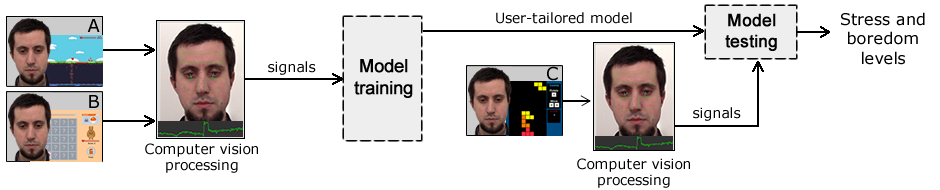
\includegraphics[width=\textwidth]{figures/machine-learning-investigation.png}
    \caption{Iteration of a 3-fold \textit{Leave One Session Out Cross Validation} performed on a gaming sessions with 3 games, i.e. A, B and C. Data of two calibration games, e.g. A and B, are used to train the machine learning model, while data of the third calibration game, e.g. C, is used to evaluate the model.}
    \label{fig:experiment2-training-evaluation}
\end{figure}

In the training process of each user-tailored model, features are extracted from video segments $H_0$ and $H_1$ (calibration data) of a given subject. The hyper-parameters of the subject's model, e.g. number of neurons, is optimized using random search \parencite{bergstra2012random}. A 10-fold cross validation method repeated 3 times is applied, so the training data is split into 10-subsets and each of those subset is held out while the model is trained on all others. The process is repeated 3 times and the final metric for the model is the mean from the number of repeats. Area under the ROC curve (AUC) is used as a metric to select the best model.

According to previous analysis, subjects perceived the calibration games as being boring at the beginning and stressful at the end. As a consequence, it is assumed that subject's emotional state in $H_0$ and $H_1$ is boredom and stress, respectively. Based on that assumption, training data obtained from video segments in $H_0$ and $H_1$ were labeled as boredom and stress, respectively.

\subsection{Construction of validation datasets}
\label{sec:experiment2-construction-validation}

The majority of the works in the literature validate an emotion classifier by applying it to a share of the samples that were not used for training. Commonly all available data samples are split in two sets, e.g. containing 80\% and 20\% of all samples, which are then used for training and validation, respectively. In such configuration, all data used in the process comes from the same source, the only difference is how it is distributed in different sets. Contrary to that approach, the evaluation of the emotion classifier proposed in this experiment has been validated using a completely different and independent dataset.

As mentioned in the previous section, data extracted from the calibration games, i.e. video segments $H_0$ and $H_1$ of a given subject $S_i$, is used to train a model $N_i$. Data extracted from the Infinite Mario game, i.e. video segments $M_i$, is sampled to produce the evaluation dataset. It is important to highlight how unique and challenging such configuration is, since the user-tailored model is trained on a dataset (calibration games) and tested/validated on another one (evaluation game). They are from completely different and independent sources. Despite that configuration, the game used for evaluation, i.e. Infinite Mario, still shares common characteristics with the calibration games, such as the 2D and casual mechanic.

The feature extraction procedure described previously uses a moving window of 15 seconds with a step of 1 second. When it is applied to the video segments $M_i$, a new value for each feature is extracted per second. It has been reported in the literature that HR-based emotion estimation is possible every 10 seconds \parencite{valenza2014revealing}, however reports also show changes in inter-beat interval of HR within 4 seconds after in-game events \parencite{ravaja20051}. Regarding facial actions, they might change faster than HR, so it is reasonable to believe they could significantly change within a time span of 10 seconds. As a consequence, a sampling of 5 seconds has been selected to collect feature values for the testing dataset of a given subject out of video segments $M_i$. A sampling of 5 seconds is expected to cover changes both in HR and facial actions as often as possible without risking to collect samples that are not independent.

The testing dataset of a given subject $S_i$ contains all samples (acquired every 5 seconds) from all levels of that given subject $S_i$ selected for evaluation. The self-reported emotional state provided by each subject in the selected levels is used as ground truth to test the accuracy of the model. The levels of Infinite Mario used for evaluation are selected according to the following procedure. Assuming that $rstress_{i,j}$ and $rboredom_{i,j}$ represent the self-reported levels of stress and boredom of subject $S_i$ in a Mario level $j$, respectively, a stress score $stress_{i,j}$ and a boredom score $boredom_{i,j}$ are calculated as:

\begin{equation}
  stress_{i,j} = rstress_{i,j} - rboredom_{i,j}
  \label{eq:stress-score}
\end{equation}

\begin{equation}
  boredom_{i,j} = rboredom_{i,j} - rstress_{i,j}
  \label{eq:boredom-score}
\end{equation}

Two Mario levels, i.e. video segments $M_i$, of a given subject $i$ with the highest values for $stress_i$ are selected and used for sampling of stress entries. Similarly the two levels with the highest values for $boredom_i$ are selected and used for sampling of boredom entries. In order to avoid the sampling of levels whose self-reported emotional state is inconclusive, e.g. stress and boredom levels are equal, levels already selected for sampling whose values of $stress_i$ or $boredom_i$ are not greater or equal to 1 are excluded from the sampling process.

\subsection{Evaluation of the emotion classifier}

Similarly to the training process, the evaluation process happens on a user basis, as illustrated by Figure \ref{fig:experiment2-training-evaluation}. After the user-tailored model $N_i$ of a given subject $S_i$ has been trained, it is applied on the testing dataset of that subject. The testing dataset of a given subject $S_i$ contains all samples (acquired every 5 seconds) from all levels of that given subject $S_i$ selected for evaluation, as described in Section \ref{sec:experiment2-construction-validation}.

The evaluation of the proposed emotion classifier is based on classification accuracy. As mentioned early, each user-tailored model $N_i$ is applied to a testing dataset sampled for that particular subject. Consequentially each subject $S_i$ produces one single accuracy metric, named $A_i$. The overall classification accuracy of the proposed method is calculated based on the mean of all $A_i$ values.

%%%%%%%%%%%%%%%%%%%%%%%%%%%%%%%%%%%%%%%%%%%%%%%%%%%%%%%%%%%%%%%%%%%%%%%%%%%%%%%%%%%%%%%
\subsection{Analysis}
%%%%%%%%%%%%%%%%%%%%%%%%%%%%%%%%%%%%%%%%%%%%%%%%%%%%%%%%%%%%%%%%%%%%%%%%%%%%%%%%%%%%%%%

The aim of the experiment is to validate and prove the feasibility of the proposed emotion detection approach, i.e. use of remotely acquired signals and a user-tailored model (trained on data from calibration games) to detect emotional states of stress and boredom. The feasibility of the approach will be tested in terms of classification accuracy.

Thus the following hypothesis is stated:

\begin{itemize}
  \item $u_1$: a user-tailored model, i.e. neural network, trained on data samples from three calibration games of a given subject $S_a$, i.e. Mushroom, Platformer and Tetris, is able to classify the emotional state of samples extracted from an evaluation game, i.e. Infinite Mario, played by that same subject $S_a$ with mean accuracy greater than chance-level rate;
\end{itemize}

Chance level is thereby the accuracy achieved assuming that it is equally likely for a data sample to fall in any of the existing classes \parencite{kassraian2016promises}. For a balanced two-class problem, chance-level classification accuracy equal 50\%. However, a chance-level accuracy rate of 50\% assumes a classifier performing random guessing on data sets of infinite size. As a consequence, random guessing approximates chance level accuracies if the testing data set is large enough. If the testing data set if small, random classification can deliver accuracies strongly deviating from chance level \parencite{combrisson2015exceeding}.

In order to account for that, a minimal correct classification rate for accuracy has been calculated using the binomial cumulative distribution to assert statistical significance with a confidence level of 95\% ($p < 0.05$) as a function of sample size $n$, i.e. size of validation dataset, and number of classes, i.e. boredom and stress \parencite{combrisson2015exceeding}. Since subjects have different gaming skills, time spent playing levels of Infinite Mario are likely to differ. It produces validation datasets of different sizes among subjects. An analysis of all validation datasets show a mean size of 64.4 samples with 32.1 and 32.3 being the mean number of stress and boredom samples in each set, respectively. Therefore it has been assumed that the proposed method is being validated as a balanced two-class problem with a sample size of $n=64$ (on average) used for the evaluation of each classification. Based on those numbers, a mean classification accuracy rate of 60\% has been found as the minimal rate to assert classification better than chance-level.

Hypothesis $u_1$ was tested by checking if the mean value of the classification accuracy, i.e. calculated from all $A_i$ values, is greater than 0.6.

%e refer the reader to Combrisson and Jerbi \parencite{combrisson2015exceeding} who explain in detail how assuming a binomial distribution for the classification error, significant classification accuracies can be calculated.

%%%%%%%%%%%%%%%%%%%%%%%%%%%%%%%%%%%%%%%%%%%%%%%%%%%%%%%%%%%%%%%%%%%%%%%%%%%%%%%%%%%%%%%
\section{Results}
%%%%%%%%%%%%%%%%%%%%%%%%%%%%%%%%%%%%%%%%%%%%%%%%%%%%%%%%%%%%%%%%%%%%%%%%%%%%%%%%%%%%%%%

The following sections present the results obtained with the analysis of the data performed according to the previously described method.

%%%%%%%%%%%%%%%%%%%%%%%%%%%%%%%%%%%%%%%%%%%%%%%%%%%%%%%%%%%%%%%%%%%%%%%%%%%%%%%%%%%%%%%
\subsection{Self-reported emotional state}

The emotional state of subjects during the interaction with the Infinite Mario game is an important element of the experiment. Table \ref{table:experiment2-mario-emotions} shows the mean value and standard deviation of the answers given in the self-reported emotional state questionnaire after each level of Infinite Mario.

\begin{table}[!htbp]
  \centering
  \caption{Mean value of the answers given in the self-reported emotional state questionnaire after levels of Infinite Mario}
  \label{table:experiment2-mario-emotions}
  \begin{tabular}{ccc}
    \hline
      \textbf{Level} & \textbf{Stress} & \textbf{Boredom} \\
    \hline
      $A_1$ & 1.6 $\pm$ 0.8 & 2.3 $\pm$ 1.2 \\
      $A_2$ & 2.1 $\pm$ 0.9 & 1.8 $\pm$ 1.1 \\
      $A_3$ & 2.9 $\pm$ 0.9 & 1.9 $\pm$ 1.2 \\
      $B_1$ & 1.5 $\pm$ 1.0 & 3.9 $\pm$ 1.2 \\
      $B_2$ & 2.0 $\pm$ 0.8 & 2.2 $\pm$ 1.2 \\
      $B_3$ & 3.0 $\pm$ 1.1 & 2.1 $\pm$ 1.2 \\
      $C_1$ & 1.3 $\pm$ 0.7 & 4.0 $\pm$ 1.2 \\
    \hline
  \end{tabular}
\end{table}

Levels $A_3$ and $B_3$ presented 2.9 and 3.0 as the mean value for reported stress, respectively, the two highest mean values for stress. Using level $A_1$ as a baseline, since it presented the lowest median values for stress and boredom, i.e. 1.0 and 2.0 respectively, a Wilcoxon Signed-ranks test indicated different stress levels between $A_1$ (median 2.0) and $A_3$ (median 3.0), $Z=-5.78$, $p < 0.001$, $r=0.73$. The same test also indicated different stress levels between $A_1$ (median 2.0) and $B_3$ (median 3.0), $Z=-5.55$, $p < 0.001$, $r=0.70$.

Levels $B_1$ and $C_1$ presented 3.9 and 4.0 as the mean value for reported boredom, respectively, the two highest mean values for boredom. Repeating the use of level $A_1$ as a baseline, a Wilcoxon Signed-ranks test indicated different boredom levels between $A_1$ (median 2.0) and $B_1$ (median 4.0), $Z=-6.14$, $p < 0.001$, $r=0.77$. The same test also indicated different boredom levels between $A_1$ (median 2.0) and $C_1$ (median 4.0), $Z=-6.21$, $p < 0.001$, $r=0.78$.

As mentioned in Section \ref{sec:experiment2-evaluation-game}, levels $A_3$ and $B_3$ were adjusted to be perceived as more stressful. Similarly levels $B_1$ and $C_1$ were adjusted to be perceived as more boring. Results with statistical significance confirm that the adjustments applied to those levels of Infinite Mario indeed caused a particular emotional state.

Such confirmation should ensure that features extracted from the video recordings of Infinite Mario gameplay are indeed associated with emotional states of stress and boredom. It is essential for the evaluation and validation of the proposed method.

%%%%%%%%%%%%%%%%%%%%%%%%%%%%%%%%%%%%%%%%%%%%%%%%%%%%%%%%%%%%%%%%%%%%%%%%%%%%%%%%%%%%%%%
\subsection{Emotion classification}

Subject's emotional state during the interaction with particular levels of Infinite Mario was classified as stress or boredom using the proposed method. Table \ref{table:experiment2-result-metrics-mean} presents the mean value of the resulting classification metrics for accuracy, precision, recall and F1 score, calculated and analyzed according to the procedures described in Section \ref{sec:experiment2-method}.

\begin{table*}[ht]
    \centering
    \caption{Mean values of resulting classification metrics}
    \label{table:experiment2-result-metrics-mean}
    \begin{tabular}[l]{@{}cccc}
        \hline
            \textbf{Accuracy} & \textbf{Precision} & \textbf{Recall} & \textbf{F1}\\
        \hline
            0.6158 & 0.6163 & 0.6127 & 0.5786 \\ % 912327a8-c86e26c6
        \hline
    \end{tabular}
\end{table*}

The proposed method was able to identify the emotional state of subjects with a mean accuracy of 61.6\%. As previously mentioned, hypothesis $u_1$ states that a user-tailored model, i.e. neural network, trained on data samples from three calibration games of a given subject $S_a$, i.e. Mushroom, Platformer and Tetris, is able to classify the emotional state of samples extracted from an evaluation game, i.e. Infinite Mario, played by that same subject $S_a$ with mean accuracy greater than 60\% (calculated chance-level rate). A mean accuracy of 61.6\% supports hypothesis $u_1$, confirming the feasibility of the proposed method to perform better than chance-level estimations.

Since subjects were evaluated independently, the mean classification accuracy is not enough to contextualize the estimations on a user level. Figure \ref{fig:experiment2-result-charts} provides a better context of the distribution of accuracy values on a subject level as observed by a histogram and density curves. As illustrated in the histogram of Figure \ref{fig:experiment2-result-charts}(a), the majority of the subjects presented an emotion classification accuracy close to 60\%. Particularly wrong estimations can be observed in a group of 13 subjects (20.9\%) that were classified with mean accuracy inferior to 50\%. Contrarily, a group of 14 subjects (22.5\%) presented particularly precise emotion estimations with classification accuracy greater than 75\%.

\begin{figure}[ht]
\centering
  \begin{subfigure}[b]{0.5\textwidth}
    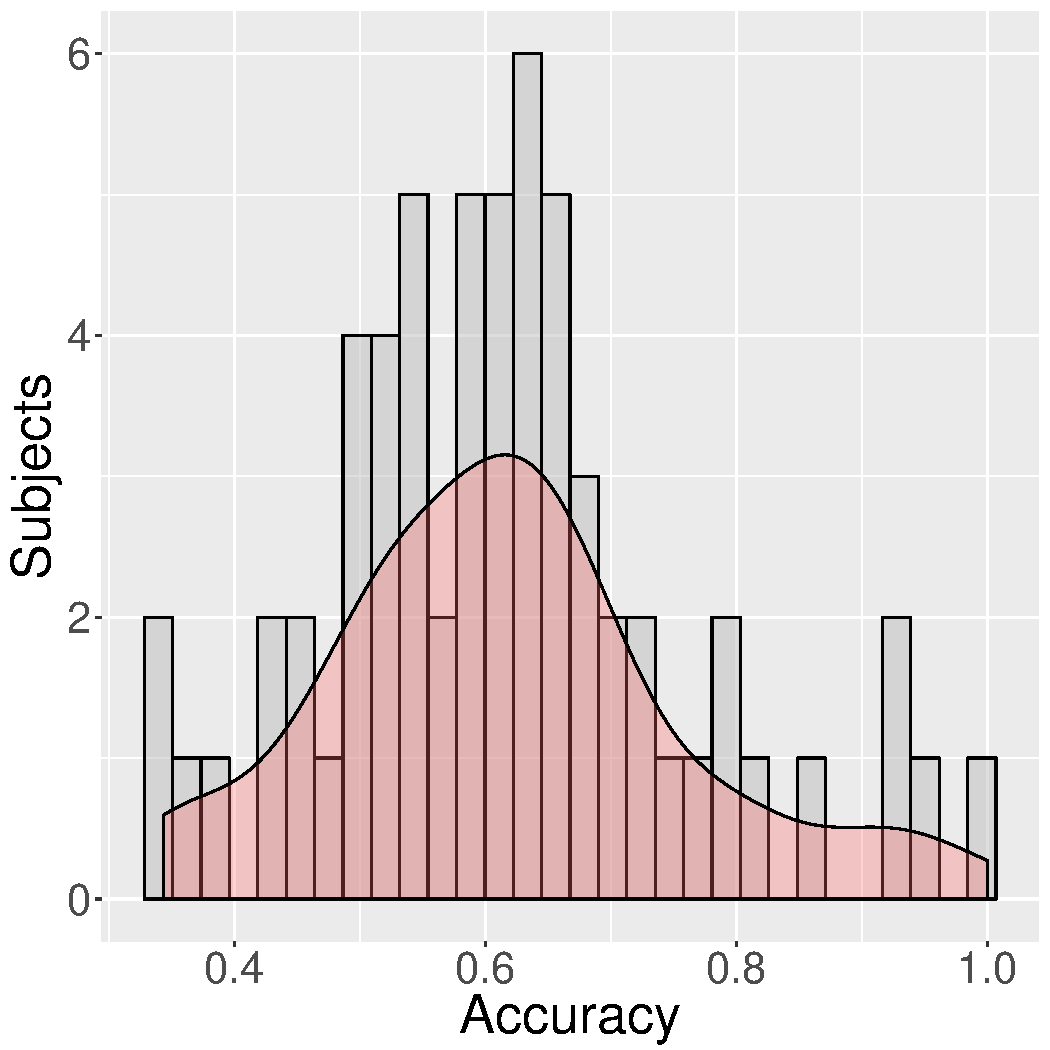
\includegraphics[width=0.95\textwidth]{figures/experiment2-hist-user}
    \caption{}
    \label{fig:experiment2-chart-hist}
  \end{subfigure}%
  \begin{subfigure}[b]{0.5\textwidth}
    \centering
    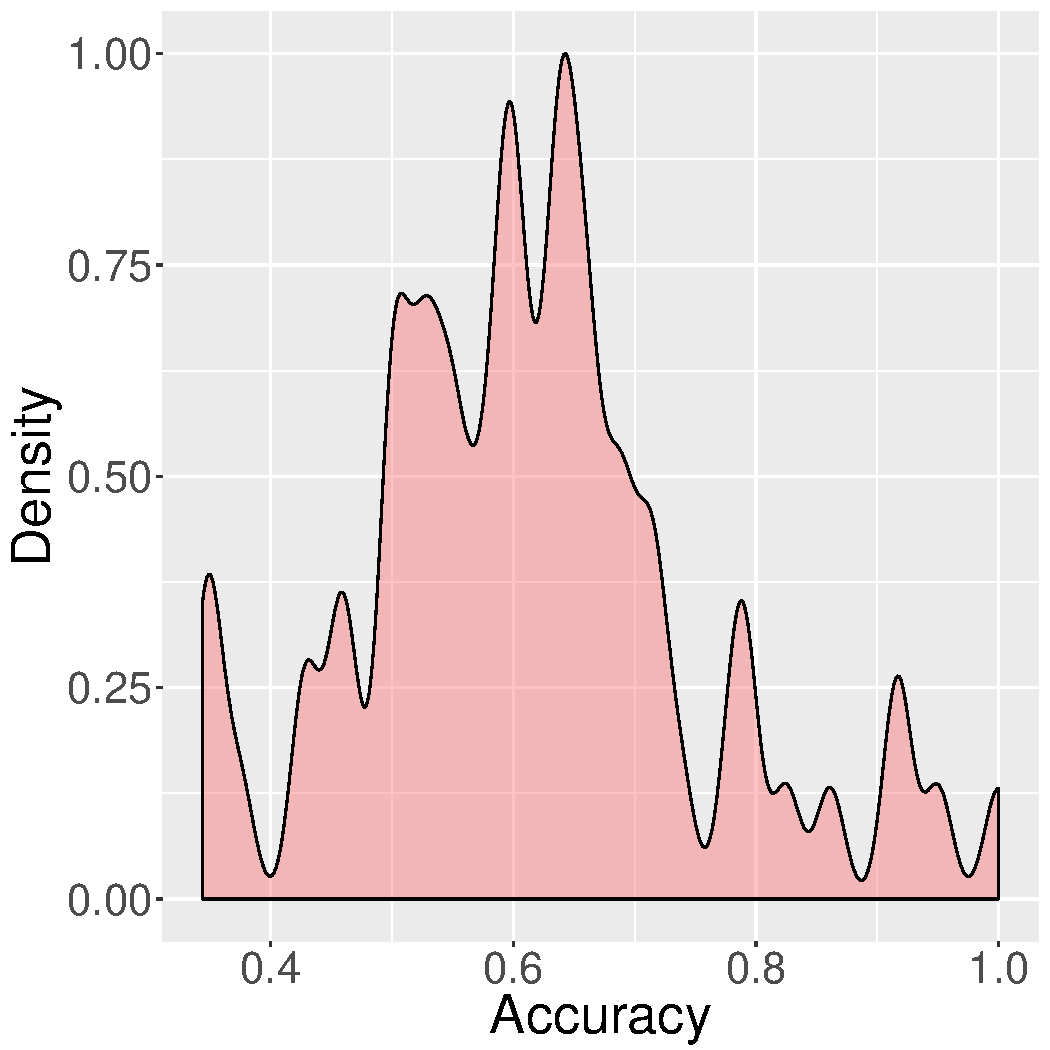
\includegraphics[width=0.95\textwidth]{figures/experiment2-density-user}
    \caption{}
    \label{fig:experiment2-chart-density}
  \end{subfigure}
  \caption{Write something nice about those here.}
  \label{fig:experiment2-result-charts}
\end{figure}

Figure \ref{fig:experiment2-result-charts}(b) shows a density curve with default bandwidth and an adjustment of 0.25 regarding the distribution of accuracy values. In such illustration, the area under any part of the curve provides the probability that the accuracy value would equal that particular group of samples. As expected, there is a greater likelihood of samples being classified with an accuracy of 60\% (mean accuracy). Interestingly is the likelihood of samples being classified with an accuracy of 80\% or 90\%, which are more likely than a classification accuracy of 40\%.


%%%%%%%%%%%%%%%%%%%%%%%%%%%%%%%%%%%%%%%%%%%%%%%%%%%%%%%%%%%%%%%%%%%%%%%%%%%%%%%%%%%%%%%
\section{Discussion}

Results of the proposed method for emotion detection based on remotely acquired signals show that the mean classification accuracy of 61.6\% is better than a calculated 60\% chance-level. As described in Section \ref{sec:experiment2-method}, the evaluation of the method has been performed as a balanced two-class problem with a sample size of $n=64$ (on average). Particularly the chance-level mean classification accuracy rate of 60\% has been found assuming a binomial distribution for the classification error to ensure a statistically significant classification \parencite{combrisson2015exceeding}. The achieved mean classification accuracy of 61.6\% supports the proposed hypothesis $u_1$, proving that a user-tailored model trained on data samples from three calibration games of a given subject is able to classify the emotional state of samples extracted from an evaluation game played by that same subject. The use of calibration games as emotion elicitation for training of an emotion classifier is a novel aspect of the method presented here. Results support such idea, showing that calibration games could be used as emotion elicitation material.

Despite the fact that a mean classification accuracy of 61.6\% is better than the calculated chance-level accuracy of 60\%, it is still below the mean classification accuracy achieved in other affective computing studies. A literature review performed by \textcite{moghimi2017affective} of over 33 affective computing studies undertaken since 1993 show a mean classification accuracy of 77.91\% ($\pm$12.76\%, minimum of 50\%, i.e. random classification, and maximum of 96.5\%). The method proposed here is within the reported range, however a fair comparison of evaluation metrics is virtually impossible considering the different methods, setups and aims. When compared in isolation, mean accuracy is a simple metric to estimate how good an approach is at classifying emotional states. However the evaluation method and the procedures used for training/testing the model can profoundly influence accuracy results. For instance, \textcite{kukolja2014comparative} classify 5 emotions using kNN (nearest neighbors) based on physiological signals obtained with physical sensors. When Leave-One-Out Cross-Validation (LOOCV) is employed, i.e. available data is divided in parts and one is left out while the rest is used for training, the mean evaluation accuracy is 78.76\%. When LOSOCV is used, i.e. one experimental session is left out for testings and the remaining ones are used for training, mean evaluation accuracy drops to 56.18\%. Studies using LOOCV usually report mean classification accuracy in the range 60-80\%, however LOOCV is less likely to be encountered in a real world situation. When the data available is divided in two groups, e.g. training and testing datasets, samples that are highly correlated, i.e. samples from the same game or session, could exist in both datasets. In the present experiment, for instance, data samples from the game being evaluated, i.e. Infinite Mario, are not in the training dataset. They are, in fact, used exclusively in the testing/evaluation dataset, which is completely indendent from the training data. Classification performance on fresh data from the validation set is a better measure for how well the classifiers generalize \parencite[Chapter 5]{james2013introduction}. Therefore the use of LOOCV, even when k-fold cross-validation is used, presents testings samples that are considerably similar to those found in the training dataset, which could lead to higher mean classification accuracy.

It is also important to highlight how the signals used in the emotion classification are acquired. In the method proposed in the present experiment, all information used to build the user-tailored model is collected remotely, in a non-obtrusive manner. Previously mentioned mean classification accuracy of 77.91\% from other affective computing studies depend on physical sensor to acquire subject's signals. A completely remote emotion estimation setup presents a significant set of challenges. When completely remote data acquisition is employed by previous studies, results show an accuracy rate of 89\% for negative, 56\% for neutral and 78\% for positive state identification \parencite{mental}. When only stress is being detected, mean classification accuracy reached best marks of 80\% and 90\% in contexts involving interactions with stressful images and the Stroop test \parencite{giannakakis2017stress}. Finally in a context involving the detection of cognitive stress, mean accuracy classification of rest vs. cognitive load has been reported as 86\% \parencite{mcduffcogcam}. All those studies rely on a completely remote method for data acquisition, however the context in which the classification is being conducted is not focused on games research or in the use of games as the source of emotion elicitation for the training of the model. Additionally, LOOCV or equivalent is used in some cases, so the model accuracy is influenced by that, as previously mentioned. As detailed in the survey by \textcite{moghimi2017affective}, there are a myriad of different experimental setups and approaches for affective computing. Given the peculiarities of each approach, including how the model is trained and evaluated, it would be unfair and naive to make a direct comparison of studies. Attention should be put on the method, aims and evaluation of any presented approach, so merit can be decided.

Finally an important factor in the present experiment is the material used to produce the emotional stimuli. Differently from previous studies, subjects were interacting with complete digital games, not images, videos or text as content to produce the emotional stimuli. The evaluation game, as well as the calibration games used in the experiment, are not gamified cognitive tests, e.g. Stroop test \parencite{golden1978stroop}. It strengthens the applicability of the results in the field of games research, which is the foundation and the aim of the proposed approach. Another remark is that a mean classification accuracy of 61.6\% might not necessarily be connected to flaws in the proposed approach, but due to limitations in the labeling of ground data. The most reliable technique to assess and label emotional experiences in order to perform appropriate psycho-physiological signal classification is self-assessment of the emotional state \parencite{moghimi2017affective}. However even if a subject reported as stressful a particular level of Infinite Mario, it does not mean that all samples collected from that level represent an emotional state of stress. It is plausible to believe that subjects experienced fluctuations of emotions during a single level, e.g. stress, happiness, and even boredom. Those nuances are not captured by the labeling process used to create the evaluation dataset, which could lead to lower classification accuracy. The heterogeneous nature of the subjects population, however, should ensure that such factor is accounted for. The considerable number of subjects in the experiment should be noted, i.e. $N=62$ is greater than the average number of participants in previous affective computing studies, which is $N=25.5$ subjects per experiment \textcite{moghimi2017affective}. It allows a broad evaluation of the proposed approach, accounting for different player profiles and supporting the claims of the previously mentioned hypothesis.

%Additionally the experiment duration varies from 20 seconds to 10 minutes and the non-game stimuli content is less likely to produce the reactions of a real gaming session, for instance spontaneous body movement and facial actions.

% \textcite{kukolja2014comparative} use a neural network and Leave-One-Session-Out Cross-Validation (LOSOCV) for emotion classification based on several physiological signals obtained with physical sensors. The authors report mean accuracy of 60.3\% in classification of 5 discreate emotions.



% Humans detect six basic emotional expressions in faces with mean accuracy of 77.3\% \parencite{bassili1979emotion}, however those facial expressions were being performed by actors (exagerated).

% A multimodal context-sensitive HCI where a clean input from a known actor cannot be expected, i.e. exaggerated facial expressions of "basic" emotions, does not suffice \parencite{pantic2003toward}.

% Additionally, the validation sampling is every 5 seconds based on \parencite{ravaja20051} (IBI with a peak decrease 4 sec after event onset) and \parencite{valenza2014revealing} (estimating emotions each 10 seconds achieve an overall accuracy in recognizing four emotional states based on the circumplex model of affect of 79.29\%, with 79.15\% on the valence axis, and 83.55\% on the arousal axis).

%%%%%%%%%%%%%%%%%%%%%%%%%%%%%%%%%%%%%%%%%%%%%%%%%%%%%%%%%%%%%%%%%%%%%%%%%%%%%%%%%%%%%%%
\section{Conclusion}

Conclude everything beautifully, showing the amount of good we are doing for the world.

%The experiment design will be based on a within-subject approach \cite{lane2015online}. In such approach, all participants perform at all levels of the treatment and there are no control groups. It is the opposite of a between-subjects approach, where subjects are divided in more than one group that receive different treatments. In that approach there are special groups, called control groups, that receive no treatment. The comparison between the control groups and the treatment groups ensures internal validity. In the context of this research, physiological signals will be measured, so the division of subjects into more than one group poses a comparison problem. Each individual will inevitably differ from one another regarding physiological signals, such as variations in average HR during rest, for instance. When measuring HR, for instance, some subjects will have higher/lower HR mean than others, independent of the group they are in or the treatment they undergo. To counter that problem, the experiment will use a one-group posttest design \cite{kirk1982experimental}, as illustrated by Figure \ref{fig:experiment}. Using the first row as an example, subject $S_0$ played game $G_a$ as the first level of the treatment, followed by a post-test of that game ($PT_a$), then a rest period. In the second level of the treatment, the subject played game $G_b$, followed by a post-test of that game ($PT_b$), then another rest period. Finally in the third level of the treatment, the subject played game $G_c$ followed by a post-test of that game ($PT_c$).

%\begin{figure}[ht]
%    \centering
%    \includegraphics[scale=0.5]{imgs/experiment-design.png}
%    \caption{One-group posttest experiment design used in this research. $S_j$ represents the $j^{\text{th}}$ subject, $G_i$ represents a game of type $i$, $PT_i$ is the post-test for game $G_i$ and $rest$ is a resting period.}
%    \label{fig:experiment}
%\end{figure}

%By using a one-group posttest design, each individual will perform on all levels of the treatment (play a set of different games). The within-subjects approach ensures that the differences between subjects are not interfering in the comparison, since a subject is being compared to his/herself in the different levels of the treatment. Subjects are not being compared among each other. In essence, each subject is serving as his/her own control group. According to Kirk \cite{kirk1982experimental}, the one-group posttest design should only be used when the researcher knows the mean value of the independent variable when no treatment is in effect. Such information will be obtained during the resting periods of the experiment, where the baseline value for all measured signals can be established for each subject.

%The process of sampling a group of participants for each experiment will follow the convenience sampling approach, a non-probability sampling technique where participants are recruited because of their convenient accessibility/proximity to the researcher. Volunteers will be randomly recruited for each experiment. A probability sampling approach, where each individual of the population has an equal chance of being selected, would be ideal and would strength the external validity of the research. However the costs, logistics and time constraints associated with it makes such approach impractical in the context of this research.







%\section{Experimental validation of the proposed method}
%\label{closing:emotion-detection-experiment}

%After the previous tasks have been completed, the limitations of the remote readings will be known (and mitigated), the set of user signals to be used in the user-tailored model will be defined and a machine learning model to map user signals into emotional states will be selected. In summary the proposed emotion detection process will be structuraly complete, but not validated.

%An experiment involving emotion detection and a commercial off-the-shelf (COTS) game will then be planned and executed to validate the proposed approach. The experiment, referred to as experiment 2 from now on, aims to test the following hypotesis (\textbf{H}):

%\textbf{H: the method proposed by this research (game-calibrated and user-tailored remote detection of emotions) is more accurate at detecting stress/boredom levels of users during the interaction with a COTS game than it is a detection approach solely based on HR measurements that are above/below the user's baseline.}

%The detection method solely based on HR, however, can use different approaches to perform the HR measurements. It can use a physical sensors, e.g. watch, or a remote approach, e.g. rPPG. In that sense, the previously mentioned hypotesis \textbf{H} can be reformulated into two hypotheses, \textbf{H1} and \textbf{H2}:

%\begin{itemize}
%  \item \textbf{H1:} the method proposed by this research is more accurate at detecting stress/boredom levels of users during the interaction with a COTS game than it is a detection approach solely based on a \textit{physical sensor} and its HR measurements that are above/below the user's baseline.
%  \item \textbf{H2:} the method proposed by this research is more accurate at detecting stress/boredom levels of users during the interaction with a COTS game than it is a detection approach solely based on \textit{remotely acquired} HR measurements that are above/below the user's baseline.
%\end{itemize}

%The proposed method relies on a multifactorial approach (see chapter \ref{ch:literature-multifactorial} for information) for emotion detection. In that approach a combination of signals, e.g. HR and facial actions, is used to improve the emotion detection. In theory, this approach should be more accurate at detecting stress/boredom levels of players than a method based on a single signal, i.e. HR, which classifies HR meaurements above the user's baseline as being an emotional state of stress (\textbf{H1}).

%The proposed method is also non-intrusive (remote), however it is significantly affected by the natural behavior of users, e.g. movement and facial activity. The use of multiple signals and the noise mitigation steps (see section \ref{sec:closing-refinement}) employed in the proposed method should make the technique more tolerant to the effects of natural behavior of users. As a consequence, the proposed method should be more accurate than a method solely based on remotely acquired HR measurements, which is more affected by natual behavior of users (\textbf{H2}).

%The test of hypotheses \textbf{H1} and \textbf{H2} will provide information regarding the feasibility of the proposed method, including its accuracy and limitations. The experiment will mark the final step of the PhD project. The thesis will present those accuracy results along with a discussion regarding how and why each part of the proposed method impacted the emotion estimation. The confirmation or refutal of hypothesis \textbf{H1} and \textbf{H2} will validate the components of the proposed method, such as the game-based calibration phase and the use of a machine learning model trained on multifactorial signals.

%Future work will derive from that analysis, since there will be room to improve and further investigate each one of the components of the process, e.g. design of calibration games, remote readings of user signals, new machine learning models, addition of new input signals to the predictive model, etc.

%\subsection{Experiment design}

%The overall idea of experiment 2 is to make subjects play three games: two calibration games and one COTS game. During the whole experiment subjects will be recored by a camera and their HR will be measured by a physical sensor, i.e. a watch.

%\begin{figure}[ht]
%   \centering
%   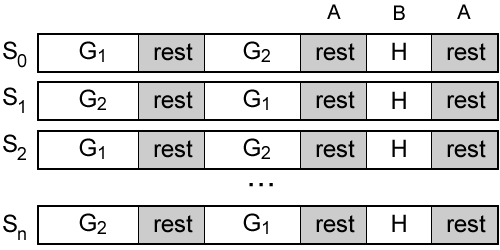
\includegraphics[width=0.6\textwidth]{figures/closing-experiment2-design.png}
%   \caption{Experimental design used in experiment 2. $S_j$ represents the $j^{\text{th}}$ subject, $G_i$ are calibration games, $COTS$ is an off-the-shelf game, and $rest$ is a resting period.}
%   \label{fig:closing-experiment2-design}
%\end{figure}

%Figure \ref{fig:closing-experiment2-design} illustrates the design of experiment 2. Each subject starts in the calibration part, where he/she plays two calibration games ($G_1$ or $G_2$) separed by a resting period (no interactions). When the subject finishes playing the calibration games, the video recordings of the subject (playing the calibration games) is processed with computer vision to extract the user signals required as input for the emotion detection model, e.g. HR and facial actions (see section \ref{sec:closing-definition-inputs}). Those extracted signals are then used to train the emotion detection model. The labeling of the signals regarding emotional states is contextualized according to the known stress and boredom aspects of the calibration games, as previously described (see sections \ref{sec:contributions} and \ref{closing:investigation-machine-learning}).

%After the model has been trained, the subject enters the emotion detection part of the experiment. In this part, the subject rests (phase A), plays a COTS game (phase B), then rests again (phase A). The video recordings of the emotion detection part is analyzed with computer vision to extract the user signals required by the emotion detection model. The extracted signals are then used as input for the previously trained emotion detection model, which outputs the estimated emotional state of the subject. The emotional state of subjects will be estimated at fixed intervals of time, e.g. every 60 seconds, throughout the emotion detection part of the experiment. Each one of those detection situations can be seen as a checkpoint. The ground truth for each checkpoint will be provided by the subjects with a self-assessment questionnaire regarding his/her current levels of stress and boredom. When a checkpoint is reached during the interaction with the COTS game, the game pauses and the questionnaire is presented to the subject. When the subject finishes answering the questionnaire, the COTS game resumes and the subject continues playing until the next checkpoint is reached.

%\begin{figure}[ht]
%    \centering
%    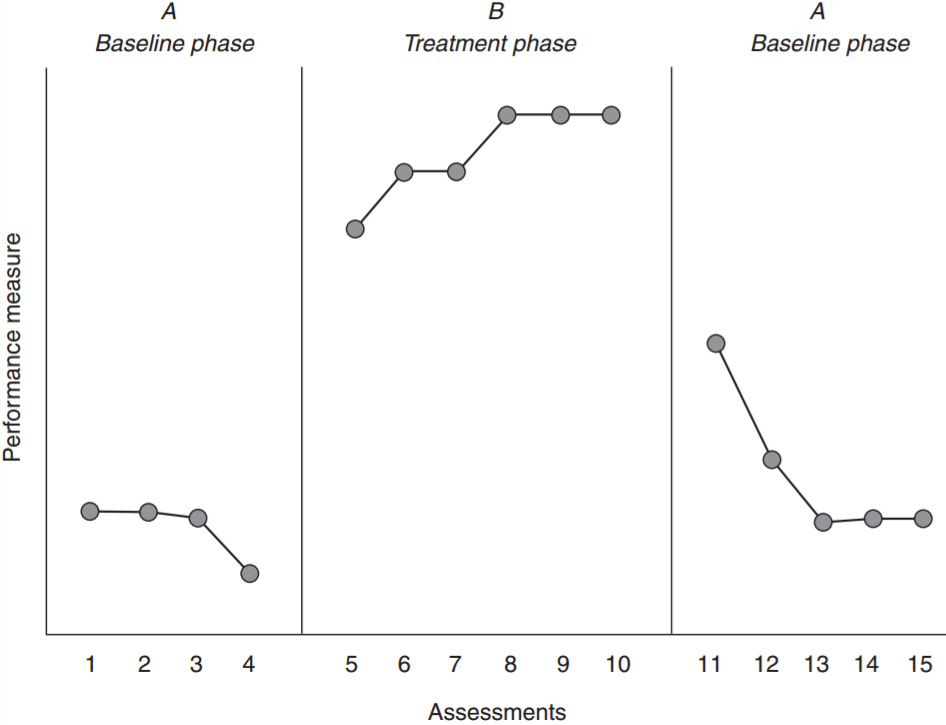
\includegraphics[width=0.85\textwidth]{figures/time-series-design-breakwell.png}
%    \caption{Time-series experimental design using an A-B-A (baseline, treatment, baseline) approach. Reproduced from \textcite{breakwell1994research}.}
%    \label{fig:time-series-design-breakwell}
%\end{figure}

%The mentioned checkpoints will be implemented using a time-series experiment design. In a time-series design there is a periodic measurement process on an individual and the introduction of a treatment into this time series of measurements results in a discontinuity in the measurements recorded in the time series \parencite{campbell2015experimental}. Figure \ref{fig:time-series-design-breakwell} illustrates the design. The A-B-A design is a common single-case time-series experimental design in which the measurements are conducted throughout the three parts of the process, i.e. A (baseline), B (treatment) and A (baseline) \parencite{robson2016real}. Phase A, referred to as the baseline phase, is a period where the subject is not under the effect of the treatment, so the measurements should reflect natural occurences. In experiment 2, it corresponds to the resting period. Phase B, referred as the treatment phase, is the period where the treatment/intervention is applied. In experiment 2, it is the interaction with the COTS game.
%In the A-B-A design, the application of a treatment followed by its removal should result in changes in the measurements among the three phases, e.g. lower values during phase A and elevated values during phase B, which confirms that the variation is a result of the treatment.

%The accuracy evaluation that confirms or refutes hypotheses \textbf{H1} and \textbf{H2} will be based on the comparison of the estimated emotional states and the self-reported emotional states informed by the subjects as ground truth during each checkpoint.

%%In the A-B-A part, the subject starts with a resting period (phase A), which is followed by the COTS treatment (phase B), finally followed by another resting period (phase A). During the A-B-A part, subjects periodically self-report their emotional state using a questionnaire, as previoslu

%%Additionally to the self-assessment of the emotional state, during the whole experiment subjects will be recorded by a video camera and monitored by a HR watch. The data collected during experiment 2 regarding the calibration games will be used to train a machine learning model, which will be used to detect the emotional state of users during the interaction with the ordinary game. The processing will be performed offline and after the experiment. Results of that analysis will prove or refute the previously mentioned hypothesis that all defined components, i.e. computer vision technique, machine learning model and calibration games, work in combination to detect emotional states.

%%During the gameplay of the non-calibration, off the shelf game the emotional state of users will be constrantly measured. Experiment 2 will produce data regarding variation of signals of subjects (from the calibration games) and ground truth data related to emotions during the gameplay of an ordinary game. The signals data will be used to train the machine learning model, which will be evaluated against the collected ground truth data (for further information regarding such validation process, see section \ref{closing:development-software}).

%%The experiment design will be based on a within-subject approach \parencite{lane2015online} where all participants perform at all levels of the treatment and there are no control groups. In the context of this research, user signals, e.g. HR, facial actions and self-reported emotional state, will be measured and used in a user-tailored model, so the division of subjects into more than one group poses a problem. Each individual will inevitably differ from one another regarding signals and emotions, such as variations in average HR during rest, for instance. Additionally people present different perceptions regarding stress and boredem. Those inherent differences pose comparision problems, so a within-subject approach simplifies the analysis of data and reduces the complexities associated with dividing subjects in different groups.

%\subsection{Challenges and unresolved issues}
%\label{experiment2-challenges}

%The first challenge regarding experiment 2 concerns the validation of the proposed method. The results of experiment 2 will demonstrate the accuracy and limitations of the proposed method, however further questioning regarding the method will innevitably surface, for instance:

%\begin{itemize}
%  \item Are all steps/signals used in the method necessary? Will a simpler and non-intrusive approach (e.g. use of remotely acquired HR information with no calibration phase) produce the same results?
%  \item Is the proposed method more accurate than an approach based on physical sensors?
%  \item Is the proposed method better than existing non-intrusive methods? It is more accurate, cheaper or easier to use?
%\end{itemize}

%Those questions could be answered with several experiments, however a direct comparison of the proposed method and existing methods is not completely plausible or viable. The proposed method relies on games as emotion elicitaion sources, which is not the case for several similar approaches that use images and sounds as stimuli. When game-like material is used as emotion elicitation sources, the context and/or the experimental design employed is different from the one proposed in experiment 2, including the use of a COTS game. Additionally a significant number of different approaches for emotion estimation exist (see chapters \ref{ch:literature-face}, \ref{ch:literature-physiological} and \ref{ch:literature-multifactorial}). Those approaches rely on different ideas, theories and signals and a direct comparison with the proposed method might not be plausible due to such differences.

%For that reason, a contextualization of the proposed method regarding existing methods is difficult. For time and resource constraints, it has been decided that an accuracy evaluation of the proposed method in comparison to a simpler emotion estimation approach based on a single signal, i.e. HR, is acceptable. It will partially answer some of the mentioned questions and provide reseachers with information to better contextualize and evaluate the feasibility of the proposed approach.

%Another challenge regarding experiment 2 is how to measure emotional states without disturbing and affecting the actual measurements. Interrupting users during gameplay is not ideal, however it is the approach described in the literature by related works. Careful planning will be required to decide the frequency and the way users will report their emotional states. If the measurements are performed too often, more data points will be available for analysis, however they might not necessarily reflect the real emotional state of users, e.g. user is bored because of the questionaire, not the game being played. If the measurements are performed too sparsely, data points will more likely reflect the real emotional state of users, however fewer data points will be available for validation.

%%Still related to emotional measurements is the decision of which questionnaire format to use in the process. As previously described, possible options are a likert scale, SAM and AS. Both SAM and AS are established and proven emotion measurement instruments, which would strengthen the theoretical foundations of the emotion measurement process. As a downside, however, they require the researcher to instruct users on how to properly answer the questionaire. User might not understand, even after the researchers explanation, what valence and arousal are, which could affect the answers and the emotion measurements. A likert scale, on the other hand, relies on the assumption that subjects know the concepts of stress and boredom within the context of games, eliminating or significantly reducing the risks of misunderstandings. If a likert scale is used, the terms ``stress" and ``boredom" can be further explained later on in the thesis using constructs of arousal and valence from established emotion theories, if that is necessary. To my understanding, a likert scale has already been successfully used in experiment 1 and is more likely to produce better results than trying to use SAM or AS as measurement tools, which risks the acquisition of answers that were misunderstood by subjects.

%Finally another unresolved issue is the COTS game to be used. Differently from the calibration games, this game should produce a natural interaction with users, causing variations of emotions that are expected from an ordinary game. The challenge is to choose a game able to elicitate sufficient variations in both boredom and stress emotional states, ortherwise the ground truth data will be skewed.

%%When measuring HR, for instance, some subjects will have higher/lower HR mean than others, independent of the group they are in or the treatment they undergo. To counter that problem, the experiment will use a one-group posttest design \cite{kirk1982experimental}, as illustrated by Figure \ref{fig:closing-experiment2-design}. Using the first row as an example, subject $S_0$ played game $G_a$ as the first level of the treatment, followed by a post-test of that game ($PT_a$), then a rest period. In the second level of the treatment, the subject played game $G_b$, followed by a post-test of that game ($PT_b$), then another rest period. Finally in the third level of the treatment, the subject played game $G_c$ followed by a post-test of that game ($PT_c$).

%%By using a one-group posttest design, each individual will perform on all levels of the treatment (play a set of different games). The within-subjects approach ensures that the differences between subjects are not interfering in the comparison, since a subject is being compared to his/herself in the different levels of the treatment. Subjects are not being compared among each other. In essence, each subject is serving as his/her own control group. According to Kirk \cite{kirk1982experimental}, the one-group posttest design should only be used when the researcher knows the mean value of the independent variable when no treatment is in effect. Such information will be obtained during the resting periods of the experiment, where the baseline value for all measured signals can be established for each subject.

%%The process of sampling a group of participants for each experiment will follow the convenience sampling approach, a non-probability sampling technique where participants are recruited because of their convenient accessibility/proximity to the researcher. Volunteers will be randomly recruited for each experiment. A probability sampling approach, where each individual of the population has an equal chance of being selected, would be ideal and would strength the external validity of the research. However the costs, logistics and time constraints associated with it makes such approach impractical in the context of this research.
